%%%%%%%% Matchovanie farieb %%%%%%%%%%
\begin{frame}{Matchovanie farieb na farby rubikovej kocky}
\begin{textblock*}{3cm}(8.5cm,3.2cm)
\uncover<2->{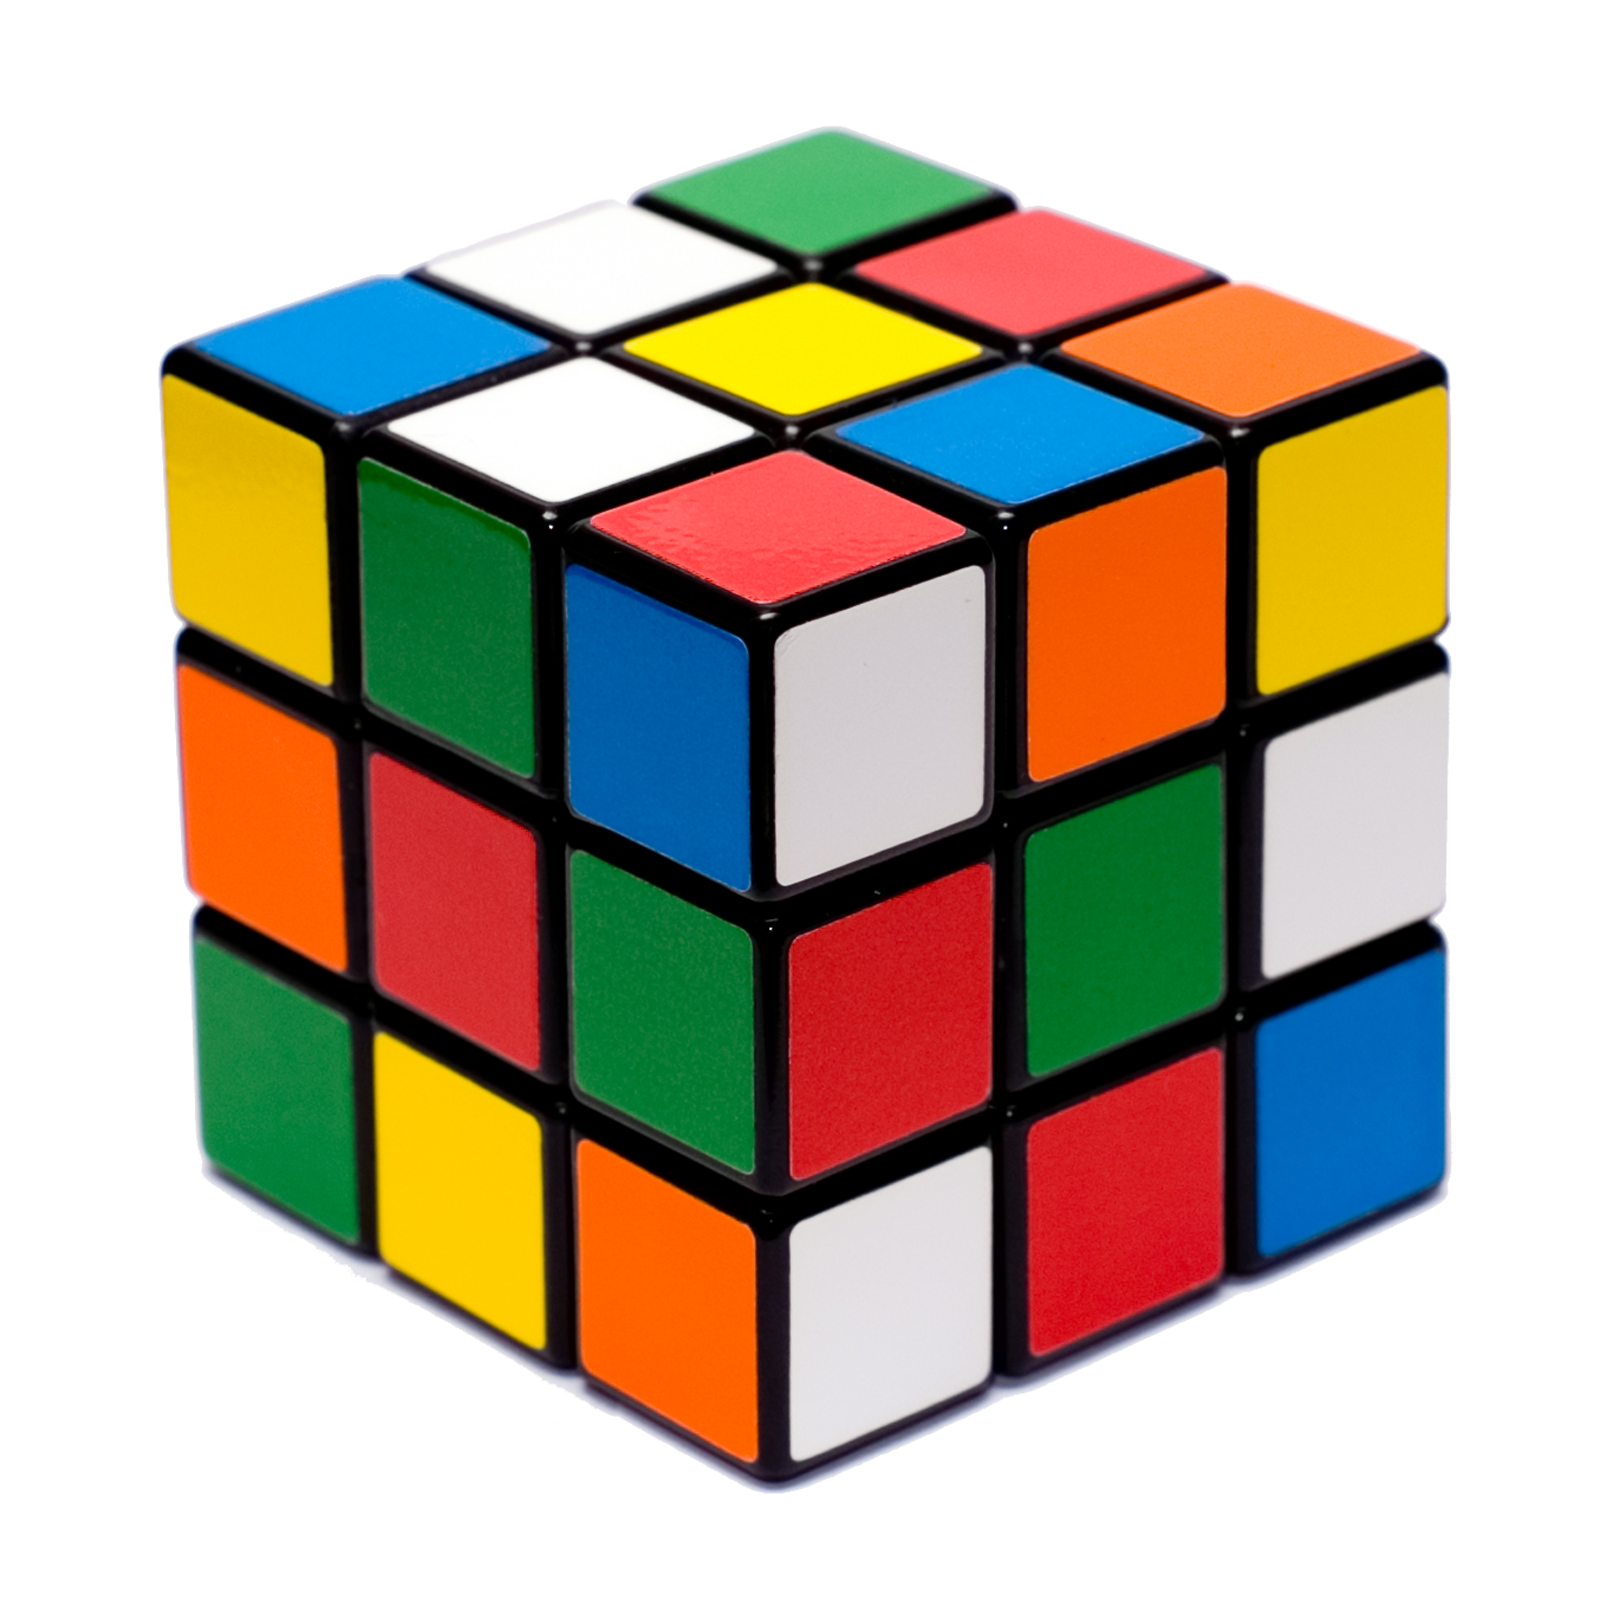
\includegraphics[width=\linewidth]{rubik}}
\end{textblock*}
\odrazka[1]{\textbf{Cieľ}: Nájdené farby priradiť k farbám originálnej Rubikovej kocky}
\begin{itemize}
\item<2->{Rubikova kocka má 6 základných farieb}
    \begin{itemize}
    \item<2-> Red: $(196, 30, 58)$
    \item<2-> Green: $(0, 158, 96)$
    \item<2-> Blue: $(0, 81, 186)$
    \item<2-> Orange: $(255, 88, 0)$
    \item<2-> Yellow: $(255, 213, 0)$
    \item<2-> White: $(255, 255, 255)$
    \end{itemize}
\end{itemize}
\odrazka[3] {Jednoduchý algoritmus pomocou matchovania farby k farbe}
\odrazka[4] {Zložitejší algoritmus pomocou zgrupovania a matchovania grupy k farbe}
\end{frame}

%%%%%%%% Matchovanie farby na farbu %%%%%%%%%%
\begin{frame}{Matchovanie 1 farby na farbu rubikovej kocky}
\begin{itemize}
\begin{textblock*}{4.5cm}(8.0cm,5.5cm)
\uncover<2->{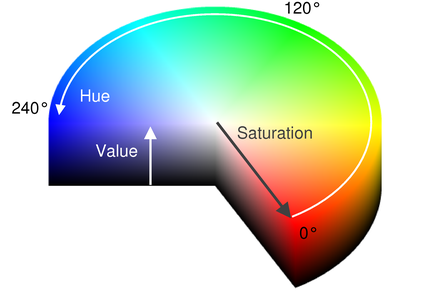
\includegraphics[width=\linewidth]{hsv}}
\end{textblock*}
\item<1->Funkcia {\tt match\_color}:
\item<2->Prevod oboch farieb do HSV
\item<3->Spočítanie skóre pre všetky farby a následný výber farby s najväčším skóre
    \begin{itemize}
    \item<4-> rozdiel 2 farieb po zložkách   
    \item<5-> výsledné skóre je váhovaný súčet zložiek
    \item<6-> pre každú cieľovú farbu sú rôzne váhy
    \end{itemize}
\end{itemize}
\end{frame}

%%%%%%%% Zgrupovanie podobných farieb %%%%%%%%%%
\begin{frame}{Zgrupovanie podobných farieb}
\begin{itemize}

\begin{textblock*}{2.5cm}(9.5cm,3.5cm)
\uncover<3->{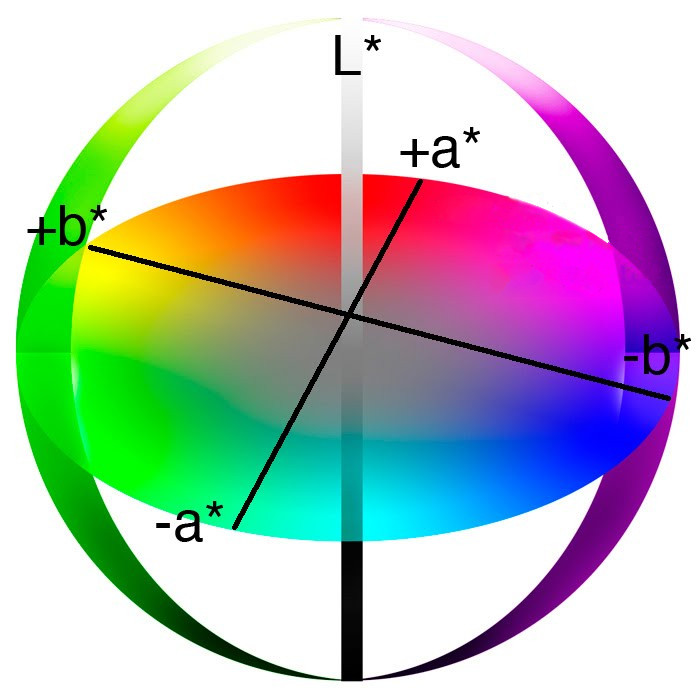
\includegraphics[width=\linewidth]{lab}}
\end{textblock*}

\item<2->Zgrupenie farieb podla podobnosti, pre každú stranu zvlášť
    \begin{itemize}
    \item<3-> prevod do $Lab$
    \item<4-> euklidovská vzdialenosť na zložkách $a$, $b$
    $$ d = \sqrt{(a_1-a_2)^2+(b_1-b_2)^2}$$
    \item<5-> treshold na vyhodnotenie podobnosti
    \end{itemize}
\item<6-> Priradenie farieb ku grupám - nájsť čo najlepšie ohodnotenie farieb, tak aby žiadne 2 grupy nemali tú istú farbu.
\end{itemize}
\end{frame}
